\chapter{System Tests}
\label{chap:6}

In this chapter, the tests  conducted to determine how well the system measures
up to the original goals and objectives set out in Sec. \ref{sec:objectives} on
p.\pageref{sec:objectives}.

The tests conducted are the system resource usage for the different payment
options and user stories where scenarios are created and the response of the
system is given. The test results are also displayed and discussed. 

\section{System Resource Usage}

Tests were conducted to check and compare the system load caused by each of the
different payment methods. The processor load, memory and disk usage were tested
by using the DStat package [\cite{website:dstat}].

The DStat software ran alongside the software being tested, which also used
some resources. However, this could not be avoided. The resource usage is
present for all three the tests, so it does not unfairly skew the results.

\subsection{Quick Response Code Test}
\label{sec:qr-tests}

\subsubsection{Processor Usage}

Fig. \ref{fig:qrcode_test_cpu} shows the total processor usage during the complete
Quick Response Code (QR Code) transaction, as described in Sec.
\ref{sec:transaction} on p.\pageref{sec:transaction}.

It can be observed from Fig. \ref{fig:qrcode_test_cpu} that there are significant spikes
near maximum capacity when the Pi starts generating a QR Code and when the return QR Code is scanned. This was expected, as
image and video processing is taxing on hardware and the Pi has no dedicated graphics
processor. The data encryption also adds to the processing load. A possible solution is to
overclock the processor, but it is already overclocked to 900 MHz and pushing the
processor harder may damage the Pi and void its warranty.

It can also be observed that there is a significant time lag between QR Code generation
and the QR Code scanning stages. This is when the user is awaiting authentication from the
server. The only way that this lag can be improved is to move the server location from the
USA to South Africa. It is not expected that doing so will make a significant
difference, however.

\begin{figure}
 \centering 
 \includegraphics[clip=true, trim = 70 260 0 70,
 scale=0.7]{qrcode_test_cpu}
 \caption{QR Code processor usage test results.}
 \label{fig:qrcode_test_cpu}
\end{figure}

\subsubsection{Disk Write Activity}

Fig. \ref{fig:qrcode_test_disk} shows the disk writing activity during the QR Code
transaction. It shows several spikes during the transaction. This can possibly be
attributed towards swap file activity by the Pi's operating system and the image encoding
and decoding processes. Optimising the code may improve this.

\begin{figure}
 \centering 
 \includegraphics[clip=true, trim = 0 530 0 70,
 scale=0.7]{qrcode_test_disk}
 \caption{QR Code disk write test results.}
 \label{fig:qrcode_test_disk}
\end{figure}

\subsubsection{Memory Usage}

Fig. \ref{fig:qrcode_test_mem} shows the memory usage during the QR Code transaction
process. It shows a relatively flat graph in the beginning, but goes up toward the end. 
It also shows that the memory used does not return to its start value. This may indicate
that memory leaks may occur over prolonged use.

The memory performance is tested and discussed in more detail in Sec.
\ref{sec:memory_leak}.

\begin{figure}
 \centering 
 \includegraphics[clip=true, trim = 0 520 0 70,
 scale=0.7]{qrcode_test_mem}
 \caption{QR Code memory usage test results.}
 \label{fig:qrcode_test_mem}
\end{figure}

\subsection{Near Field Communication Test}

\subsubsection{Processor Usage}

Fig. \ref{fig:nfc_test_cpu} shows the processor activity during the complete Near
Field Communication (NFC) transaction process. It shows an average load of approximately
50\% during the NFC scanning process. It can also be observed that the transaction takes
under a third of the time it takes for the QR Code option. This is a significant
improvement over the QR Code payment option, but code optimisation and improvements to
the Android application may improve this further.

\begin{figure}
 \centering 
 \includegraphics[clip=true, trim = 0 500 0 70,
 scale=0.7]{nfc_test_cpu}
 \caption{NFC processor usage test results.}
 \label{fig:nfc_test_cpu}
\end{figure}

\subsubsection{Disk Write Activity}

Fig. \ref{fig:nfc_test_disk} shows the disk activity during the NFC transaction process.
It shows far less spikes during the transaction than the QR Code option.  These spikes may
again be attributed toward swap file activity from the Pi's operating system.
The spikes may be fewer because of the decreased processing load and that it
takes less time to complete one transaction.

\begin{figure}
 \centering 
 \includegraphics[clip=true, trim = 0 530 0 70,
 scale=0.7]{nfc_test_disk}
 \caption{NFC disk write test results.}
 \label{fig:nfc_test_disk}
\end{figure}

\subsubsection{Memory Usage}
\label{sec:nfc_mem}

Fig. \ref{fig:nfc_test_mem} shows the memory usage during the NFC payment process. It
shows a relatively flat line, which indicates that the NFC transaction process is not
memory intensive. This is again a significant improvement over the QR Code option. 

\begin{figure}
 \centering 
 \includegraphics[clip=true, trim = 0 510 0 70,
 scale=0.7]{nfc_test_mem}
 \caption{NFC memory usage test results.}
 \label{fig:nfc_test_mem}
\end{figure}

\subsection{Stellenbosch University Card Test}

\subsubsection{Processor Usage}

Fig. \ref{fig:su_test_cpu} shows the processor usage during the Stellenbosch University
(SU) card transaction process. It shows only a single spike at 35\% while it is
scanning for a card. This is far less that the QR Code option and a small
improvement over the NFC option. This increase in performance over the NFC
option may be due to the fact that NfcPy (the module used during the NFC
transaction process) is built on top op libnfc and incorporates additional
communication protocols, making it a bulkier process than the SU card option,
which only uses the libnfc module process. The SU transaction process makes use
of only libnfc and will therefore most likely be less processor intensive.

\begin{figure}
 \centering 
 \includegraphics[clip=true, trim = 0 530 0 70,
 scale=0.7]{su_test_cpu}
 \caption{SU Card processor usage test results.}
 \label{fig:su_test_cpu}
\end{figure}

\subsubsection{Disk Write Activity}

Fig. \ref{fig:su_test_disk} shows the disk writing activity of the SU transaction
process.  It looks similar to the NFC transaction disk activity from Fig.
\ref{fig:nfc_test_disk}. This may be because they work in a similar manner and both use
libnfc to scan for NFC devices.

\begin{figure}
 \centering 
 \includegraphics[clip=true, trim = 0 550 80 70,
 scale=0.7]{su_test_disk}
 \caption{SU Card disk write test results.}
 \label{fig:su_test_disk}
\end{figure}

\subsubsection{Memory Usage}

Fig. \ref{fig:su_test_mem} shows the memory usage during the SU card transaction
process. 

With the exception of the start-up spike, the graph shows a very flat line. This indicates
that the memory usage relatively low and is very stable. 

\begin{figure}
 \centering 
 \includegraphics[clip=true, trim = 0 550 80 70,
 scale=0.7]{su_test_mem}
 \caption{SU Card memory usage test results.}
 \label{fig:su_test_mem}
\end{figure}

\subsection{Conclusions}

The resource usage of the QR Code, NFC and SU card transaction processes were analysed. It
was found that the QR Code option is the most memory and process intensive and causes
significant disk activity to take place. 

The NFC and SU card transactions cause similar system loads with regards to memory usage
and disk activity, possibly due to their common code base. However, the SU card
transaction process demands approximately 15\% less processing power than the NFC option. 

All three transaction processes can be improved and streamlined. This can be done by
porting the Python code over to compiled code format, such as C or C++. Furthermore,  some
hardware modifications, such as processor overclocking, may also decrease the system load.

\section{Usage Over Extended Period}
\label{sec:memory_leak}

This test was performed to measure the memory usage of the VM program over an extended
period of time. In this case, the VM program was left running for approximately 4.5 hours.
During this time, 8 QR Code transactions took place. 

The reason for only using QR Code transactions is because it was found that the QR
Code transaction process is the most resource intensive (see Sec. \ref{sec:qr-tests}).
Fig. \ref{fig:qrcode_test_mem} also showed that the process does not release the memory it
used during the transaction back to the system. This is called `memory leaking'.

A graph of the memory usage over time can be observed in Fig. \ref{fig:long-test}.

\begin{figure}
 \centering 
 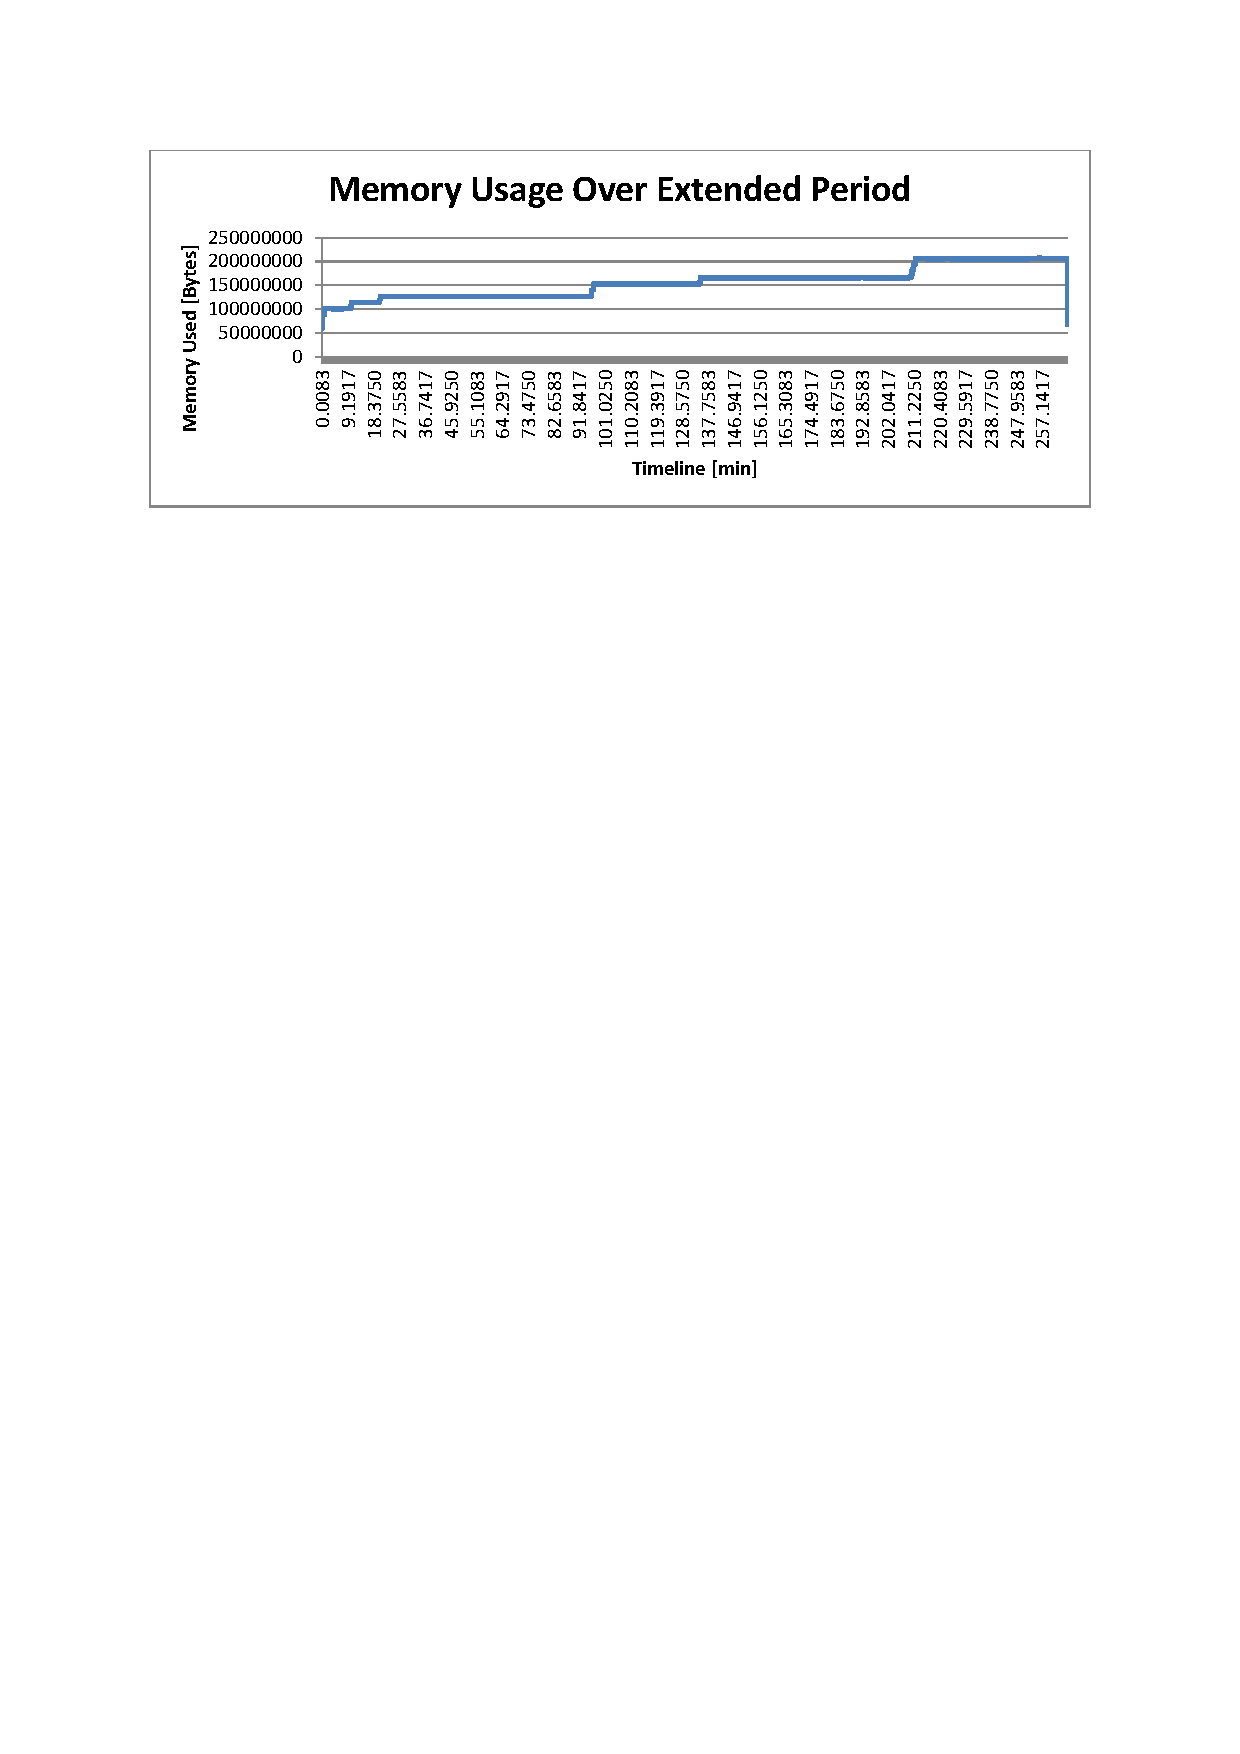
\includegraphics[clip=true, trim = 50 590 0 70,
 scale=0.9]{extended_test}
 \caption{Memory usage over extended period of time.}
 \label{fig:long-test}
\end{figure}

Fig. \ref{fig:long-test} shows that the memory usage doubles from 100 MB to 200 MB in less
than 5 hours and 8 QR Code transactions. The sudden decrease in the end is because the VM
program was shut down. 

It is suspected that the reason for this memory leakage is that the image processing step
does not properly clear after it has finished scanning a QR Code. Every subsequent QR Code
scanning process adds to this build-up of uncleared memory. This will continue until the
VM eventually runs out of memory and freezes. This may have unforeseen consequences for
the VM. 

The memory leakage here is a serious issue and must be fixed before the system can ever be
commercialised. To fix it, the code must be thoroughly inspected and tested for bugs.
This may require a possible rewrite of the image processing code. 

\section{User Tests}

The functionality of the system was tested by exposing it to different user
scenarios and seeing what the outcome was. The testing process, scenarios and
results are discussed in this section.

\subsection{User Test 1}

In this user story, the customer decides to pay with a QR Code.
He does not yet have a user account on the database and has no credits loaded.
Fig. \ref{fig:test1} shows the user story diagram. 

\begin{figure}
 \centering 
 \includegraphics[clip=true, trim = 0 410 0 60,
 scale=0.7]{user_story_1}
 \caption{The first user scenario.}
 \label{fig:test1}
\end{figure}

\subsubsection{Scenario Walkthrough}

The user first selects which product to buy from the Raspberry
Pi's User Interface (GUI). The Pi then generates a QR Code that the
user scans with any barcode scanning application. The Universal Resource Locator (URL)
embedded in the QR Code then takes the customer to a web page located on the server. 

Not having a user account, the user clicks on the link to create a new user
profile. After entering valid user information, the customer is returned to the login  page where he
can log in with his new login credentials. After logging in, the server
displays to the customer that he does not have any credits loaded onto his
account. The customer then goes to the load credit page where he loads some
money. When this is done, the server displays a confirmation QR Code on the
customer's cellphone screen, verifying the transaction.

The customer then presses the continue button on the GUI, which starts scanning the web
cam feed for the customer's QR Code. After this is done, the Pi activates the correct
motor and dispenses the product.

\subsubsection{Results}

In this scenario, a customer successfully loaded credits onto his account and bought a
product with the new credits. There are many steps involved in the process, however, and
this leads to a relatively long transaction process. 

It was also found that the server is sometimes unable to correctly decrypt the code it
receives from the customer's cellphone. It is unclear why this happens. It is
possible that the barcode scanning application on the cellphone incorrectly decodes the
VM's QR Code. This issue will have to be fixed before the system can be
commercialised.

\subsection{User Test 2}

In this scenario, a customer tries to use a QR Code from a previous transaction
without paying. Fig. \ref{fig:test2} shows the user story.

\begin{figure}
 \centering 
 \includegraphics[clip=true, trim = 0 550 0 70,
 scale=0.7]{user_story_2}
 \caption{The second user scenario.}
 \label{fig:test2}
\end{figure}

\subsubsection{Scenario Walkthrough}

To begin, the customer selects a product to buy, after which the Raspberry Pi displays a
QR Code. However, instead of scanning the QR Code and paying for a new product, the
customer tries to use an old QR Code that the server sent him after a successful
transaction previously. The customer tells the Raspberry Pi to scan his old QR
Code. The Raspberry Pi does this, but the old QR Code does not contain a valid
response to the Raspberry Pi's challenge. Therefore, the transaction is not
accepted and the customer is informed of his invalid QR Code.

\subsubsection{Results}

The results from this scenario shows that the challenge-response system works as it was
designed to: it does not allow an old QR Code to be used again without it being paid for. 

\subsection{User Test 3}

In this scenario, the user opts to buy a product using the Android NFC
application. However, the application must first be downloaded, installed and a
new user profile must be created. The user story can be seen in Fig.
\ref{fig:test3}.

\begin{figure}
 \centering 
 \includegraphics[clip=true, trim = 0 450 0 70,
 scale=0.7]{user_story_3}
 \caption{The third user scenario.}
 \label{fig:test3}
\end{figure}

\subsubsection{Scenario Walkthrough}

After the user opens the application, he is presented with a login screen. The
user enters his login credentials and checks the box that confirms that he is a
new user. The application then contacts the server with a user creation
request. Provided the username is not already used, the server creates and
saves the new user profile.

The application then takes the user to the main menu where the user can pick
a product to buy. After picking a product, the application contacts the server
with a purchase request. If the transaction is successful, the server sends the
application a confirmation code which the application transmits via the
cellphone's NFC antenna.

The user then swipes his phone across the VMs NFC receiver. The
VM then activates the motor and the user receives his product. 

\subsubsection{Results}

In this scenario, a customer has successfully used the Android NFC payment application to
create a new user profile and buy a product from the VM. 

The process is more streamlined than the QR Code option and consists of fewer steps. This
makes the NFC transaction process take place in a shorter period of time. After the
customer has opened the application once, he will not have to enter his login details
again. This will make the process slightly quicker in the future.  